\graphicspath{ {images/} }

\titledquestion{Analyzing NMT Systems}[29]

\begin{parts}

    \part[3] Look at the {\monofam{src.vocab}} file for some examples of phrases and words in the source language vocabulary. When encoding an input Mandarin Chinese sequence into ``pieces'' in the vocabulary, the tokenizer maps the sequence to a series of vocabulary items, each consisting of one or more characters (thanks to the {\monofam{sentencepiece}} tokenizer, we can perform this segmentation even when the original text has no white space). Given this information, how could adding a 1D Convolutional layer after the embedding layer and before passing the embeddings into the bidirectional encoder help our NMT system? \textbf{Hint:} each Mandarin Chinese character is either an entire word or a morpheme in a word. Look up the meanings of 电, 脑, and 电脑 separately for an example. The characters 电 (electricity) and  脑 (brain) when combined into the phrase 电脑 mean computer.

    \ifans{
        As we can see from the hint, in Mandarin Chinese, words are often composed of multiple characters, each of which
        carries its own meaning. However, when tokenized with SentencePiece, these characters are treated as separate
        subword units, potentially losing the compositional meaning of multi-character words (e.g., 电 "electricity" and
        脑 "brain" together form 电脑 "computer").

        A 1D Convolutional layer after the embedding layer helps address this issue by capturing local character-level
        patterns before passing representations to the bidirectional encoder. The convolution acts as a feature
        extractor, learning to combine adjacent token embeddings into richer representations that better reflect
        meaningful word-level structures. This is especially useful in Chinese, where token boundaries are often
        ambiguous, and a convolution can smooth out inconsistencies introduced by tokenization.
    }\fi



    \part[8] Here we present a series of errors we found in the outputs of our NMT model (which is the same as the one you just trained). For each example of a reference (i.e., `gold') English translation, and NMT (i.e., `model') English translation, please:
    
    \begin{enumerate}
        \item Identify the error in the NMT translation.
        \item Provide possible reason(s) why the model may have made the error (either due to a specific linguistic construct or a specific model limitation).
        \item Describe one possible way we might alter the NMT system to fix the observed error. There are more than one possible fixes for an error. For example, it could be tweaking the size of the hidden layers or changing the attention mechanism.
    \end{enumerate}
    
    Below are the translations that you should analyze as described above. Only analyze the underlined error in each sentence. Rest assured that you don't need to know Mandarin to answer these questions. You just need to know English! If, however, you would like some additional color on the source sentences, feel free to use a resource like \url{https://www.archchinese.com/chinese_english_dictionary.html} to look up words. Feel free to search the training data file to have a better sense of how often certain characters occur.

    \begin{subparts}
        \subpart[2]
        \textbf{Source Sentence:} 罪犯们其后被警方拘捕及被判处盗窃罪名成立。\newline
        \textbf{Reference Translation:} \textit{\underline{the culprits were} subsequently arrested and convicted.}\newline
        \textbf{NMT Translation:} \textit{\underline{the culprit was} subsequently arrested and sentenced to theft.}
        
        \ifans{
            \textbf{Error Analysis:} The mistake in the translation is the incorrect use of the singular noun “culprit”
            instead of the plural “culprits.” Since this changes the subject's number, the verb also shifts from “were”
            (plural) to “was” (singular), making the sentence grammatically incorrect.

            \textbf{Possible Causes:} The error suggests that the model struggles
            to determine whether the subject is singular or plural. This could be because the source sentence does not
            explicitly indicate plurality, making it difficult for the model to infer the correct form in English.
            Additionally, the model's attention mechanism may not have correctly captured the full subject phrase,
            or it may have been biased by training data where singular forms were more common.

            \textbf{Potential Fix:} A possible solution is improving the attention mechanism to ensure better context
            awareness when generating nouns and verbs. This could include using a more advanced self-attention model
            (such as Transformers) that can better track number agreement. Another approach is data augmentation,
            adding contrastive training examples that explicitly contain singular/plural variations to improve model
            robustness.
        }\fi



        \subpart[2]
        \textbf{Source Sentence}: 几乎已经没有地方容纳这些人,资源已经用尽。\newline
        \textbf{Reference Translation}: \textit{there is almost no space to accommodate these people, and resources have run out.   }\newline
        \textbf{NMT Translation}: \textit{the resources have been exhausted and \underline{resources have been exhausted}.}
        
        \ifans{
            \textbf{Error Analysis:} The NMT translation contains a repetition error, where the phrase “resources
            have been exhausted” is duplicated instead of fully translating the original sentence. Additionally,
            the first part of the source sentence is missing, leading to an incomplete translation.

            \textbf{Possible Causes:} A likely reason for this error is that the attention mechanism over-focused on
            one part of the source sentence, causing the decoder to repeat the phrase rather than progressing through
            the full translation. Another possible cause is exposure bias, where the model has frequently seen similar
            phrases in training and defaults to repeating them. While weak encoder representations can
            sometimes contribute to repetition errors, the bidirectional LSTM encoder should typically preserve
            context well for short sentences like this.

            \textbf{Potential Fix:} One way to fix this issue is by improving the attention mechanism to ensure
            better coverage of the entire sentence. Additionally, improving training data diversity can help the model
            generalize better and avoid defaulting to high-frequency patterns.
        }\fi


        \subpart[2]
        \textbf{Source Sentence}: 当局已经宣布今天是国殇日。 \newline
        \textbf{Reference Translation}: \textit{authorities have announced \underline{a national mourning today.}}\newline
        \textbf{NMT Translation}: \textit{the administration has announced \underline{today's day.}}
        
        \ifans{
            \textbf{Error Analysis:} The NMT translation fails to include the key phrase “national mourning,” instead
            producing an overly generic phrase, “today's day.” While the model correctly captures the announcement
            happening today, it omits the specific event, altering the meaning of the sentence.

            \textbf{Possible Causes:} One likely reason for this error is that “national mourning” is underrepresented
            in the training data, making the model less likely to generate it during translation. Another possible cause
            is that the encoder's hidden size may be too small, limiting its ability to fully represent the phrase and
            causing the decoder to lack sufficient contextual information to predict the specific event accurately.

            \textbf{Potential Fix:} One way to address this issue is by increasing the hidden layer size to improve
            the model's capacity to encode longer, less frequent phrases. Additionally, improving training data diversity
            by including more examples of “national mourning” can help the model learn the correct translation. Another
            approach is using pretrained embeddings to better capture rare or domain-specific terms.
        }\fi

        
        \subpart[2] 
        \textbf{Source Sentence\footnote{This is a Cantonese sentence! The data used in this assignment comes from GALE Phase 3, which is a compilation of news written in simplified Chinese from various sources scraped from the internet along with their translations. For more details, see \url{https://catalog.ldc.upenn.edu/LDC2017T02}. }:} 俗语有云:``唔做唔错"。\newline
        \textbf{Reference Translation:} \textit{\underline{`` act not, err not "}, so a saying goes.}\newline
        \textbf{NMT Translation:} \textit{as the saying goes, \underline{`` it's not wrong. "}}

        \ifans{
            \textbf{Error Analysis:} The NMT model correctly identified that the source sentence contains a saying,
            but it failed to translate the idiom accurately. Instead of generating the expected translation “act not,
            err not,” it produced a literal approximation, “it's not wrong,” which does not fully capture the intended
            meaning.

            \textbf{Possible Causes:} This issue arises due to both linguistic and architectural limitations. Idioms
            are \textit{non-compositional}, meaning their meaning cannot be derived directly from individual words.
            Standard sequence-to-sequence models, particularly LSTMs, struggle with such expressions because they
            process words sequentially rather than as fixed units of meaning. If the idiom appears infrequently in
            the training data, the model may not develop a strong enough representation to generate the correct
            translation. Additionally, if the hidden layer size is too small, the encoder may not effectively capture
            the idiom's meaning, causing the decoder to default to a more generic phrase.

            \textbf{Potential Fix:} A straightforward way to improve idiom translation is by increasing the diversity
            of training data, ensuring the model sees more idiomatic expressions and their correct translations.
            Fine-tuning the model on an idiom-rich dataset could also help. Some approaches outside of what I've
            explored include phrase-based lookup systems or hybrid models that handle idioms separately, but I am not
            as familiar with these techniques.

            \textbf{Extra Note:} Maybe this idiom might capture meaning from an idiom from English, such as ``You miss all the shots you don't take,''
            but the NMT model did not attempt an idiomatic translation. Instead, it produced a generic phrase
            (``it's not wrong''), likely due to a lack of exposure to idiomatic mappings in training.
        }\fi
    \end{subparts}


    \part[14] BLEU score is the most commonly used automatic evaluation metric for NMT systems. It is usually calculated across the entire test set, but here we will consider BLEU defined for a single example.\footnote{This definition of sentence-level BLEU score matches the \texttt{sentence\_bleu()} function in the \texttt{nltk} Python package. Note that the NLTK function is sensitive to capitalization. In this question, all text is lowercased, so capitalization is irrelevant. \\ \url{http://www.nltk.org/api/nltk.translate.html\#nltk.translate.bleu_score.sentence_bleu}
    } 
    Suppose we have a source sentence $\bs$, a set of $k$ reference translations $\br_1,\dots,\br_k$, and a candidate translation $\bc$. To compute the BLEU score of $\bc$, we first compute the \textit{modified $n$-gram precision} $p_n$ of $\bc$, for each of $n=1,2,3,4$, where $n$ is the $n$ in \href{https://en.wikipedia.org/wiki/N-gram}{n-gram}:
    \begin{align}
        p_n = \frac{ \displaystyle \sum_{\text{ngram} \in \bc} \min \bigg( \max_{i=1,\dots,k} \text{Count}_{\br_i}(\text{ngram}), \enspace \text{Count}_{\bc}(\text{ngram}) \bigg) }{\displaystyle \sum_{\text{ngram}\in \bc} \text{Count}_{\bc}(\text{ngram})}
    \end{align}
     Here, for each of the $n$-grams that appear in the candidate translation $\bc$, we count the maximum number of times it appears in any one reference translation, capped by the number of times it appears in $\bc$ (this is the numerator). We divide this by the number of $n$-grams in $\bc$ (denominator). \newline 

    Next, we compute the \textit{brevity penalty} BP. Let $len(c)$ be the length of $\bc$ and let $len(r)$ be the length of the reference translation that is closest to $len(c)$ (in the case of two equally-close reference translation lengths, choose $len(r)$ as the shorter one). 
    \begin{align}
        BP = 
        \begin{cases}
            1 & \text{if } len(c) \ge len(r) \\
            \exp \big( 1 - \frac{len(r)}{len(c)} \big) & \text{otherwise}
        \end{cases}
    \end{align}
    Lastly, the BLEU score for candidate $\bc$ with respect to $\br_1,\dots,\br_k$ is:
    \begin{align}
        BLEU = BP \times \exp \Big( \sum_{n=1}^4 \lambda_n \log p_n \Big)
    \end{align}
    where $\lambda_1,\lambda_2,\lambda_3,\lambda_4$ are weights that sum to 1. The $\log$ here is natural log.
    \newline
    \begin{subparts}
        \subpart[5] Please consider this example: \newline
        Source Sentence $\bs$: \textbf{需要有充足和可预测的资源。} 
        \newline
        Reference Translation $\br_1$: \textit{resources have to be sufficient and they have to be predictable}
        \newline
        Reference Translation $\br_2$: \textit{adequate and predictable resources are required}
        
        NMT Translation $\bc_1$: there is a need for adequate and predictable resources
        
        NMT Translation $\bc_2$: resources be sufficient and predictable to
        
        Please compute the BLEU scores for $\bc_1$ and $\bc_2$. Let $\lambda_i=0.5$ for $i\in\{1,2\}$ and $\lambda_i=0$ for $i\in\{3,4\}$ (\textbf{this means we ignore 3-grams and 4-grams}, i.e., don't compute $p_3$ or $p_4$). When computing BLEU scores, show your work (i.e., show your computed values for $p_1$, $p_2$, $len(c)$, $len(r)$ and $BP$). Note that the BLEU scores can be expressed between 0 and 1 or between 0 and 100. The code is using the 0 to 100 scale while in this question we are using the \textbf{0 to 1} scale. Please round your responses to 3 decimal places. 
        \newline
        
        Which of the two NMT translations is considered the better translation according to the BLEU Score? Do you agree that it is the better translation?
        
        \ifans{
            \textbf{Step-by-Step BLEU Score Calculation}

            \textbf{For $\bc_1$:}

            Unigram precision:
            $$ p_1 = \frac{0 + 0 + 0 + 0 + 0 + 1 + 1 + 1 + 1}{9} = 0.444 $$

            Bigram precision:
            $$ p_2 = \frac{0 + 0 + 0 + 0 + 0 + 1 + 1 + 1}{8} = 0.375 $$

            Brevity Penalty:
            Since $len(c_1) = 9$ and $len(r) = 7$,
            $$ BP = 1 $$

            BLEU score:
            $$ BLEU = BP \times \exp \left( 0.5 \log p_1 + 0.5 \log p_2 \right) $$
            $$ = 1 \times \exp \left( 0.5 \log(0.444) + 0.5 \log(0.375) \right) $$
            $$ = \exp(-0.8965) = 0.408 $$

            \textbf{For $\bc_2$:}

            Unigram precision:
            $$ p_1 = \frac{1 + 1 + 1 + 1 + 1 + 1}{6} = 1.0 $$

            Bigram precision:
            $$ p_2 = \frac{0 + 1 + 1 + 1 + 0}{5} = 0.6 $$

            Brevity Penalty:
            Since $len(c_2) = 6$ and $len(r) = 6$,
            $$ BP = 1 $$

            BLEU score:
            $$ BLEU = BP \times \exp \left( 0.5 \log p_1 + 0.5 \log p_2 \right) $$
            $$ = 1 \times \exp \left( 0.5 \log(1.0) + 0.5 \log(0.6) \right) $$
            $$ = \exp(-0.256) = 0.775 $$

            \textbf{Final BLEU Scores:}
            $$ BLEU(\bc_1) = 0.408, \quad BLEU(\bc_2) = 0.775 $$

            Thus, according to BLEU, $\bc_2$ is considered the better translation.

            I do not agree that $\bc_2$ is the better translation. While BLEU assigns it a higher score, a human
            evaluation reveals that $\bc_1$ is grammatically more correct and better preserves the meaning present in
            both reference translations. In contrast, $\bc_2$ is incomplete and fails to fully convey the intended
            message. This highlights a limitation of BLEU: it relies solely on n-gram precision and brevity, without
            assessing fluency or semantic accuracy.

        }\fi

        
        \subpart[5] Our hard drive was corrupted and we lost Reference Translation $\br_1$. Please recompute BLEU scores for $\bc_1$ and $\bc_2$, this time with respect to $\br_2$ only. Which of the two NMT translations now receives the higher BLEU score? Do you agree that it is the better translation?
        
        \ifans{
            \textbf{Step-by-Step BLEU Score Calculation (Using Only $r_2$)}

            \textbf{For $\bc_1$:}

            Unigram precision:
            $$ p_1 = \frac{0 + 0 + 0 + 0 + 0 + 1 + 1 + 1 + 1}{9} = 0.444 $$

            Bigram precision:
            $$ p_2 = \frac{0 + 0 + 0 + 0 + 0 + 1 + 1 + 1}{8} = 0.375 $$

            Brevity Penalty:
            Since $len(c_1) = 9$ and $len(r) = 6$,
            $$ BP = 1 $$

            BLEU score:
            $$ BLEU = BP \times \exp \left( 0.5 \log p_1 + 0.5 \log p_2 \right) $$
            $$ = 1 \times \exp \left( 0.5 \log(0.444) + 0.5 \log(0.375) \right) $$
            $$ = \exp(-0.8965) = 0.408 $$

            \textbf{For $\bc_2$:}

            Unigram precision:
            $$ p_1 = \frac{1 + 1 + 0 + 1 + 0 + 0}{6} = 0.5 $$

            Bigram precision:
            $$ p_2 = \frac{0 + 1 + 1 + 0 + 0}{5} = 0.2 $$

            Brevity Penalty:
            Since $len(c_2) = 6$ and $len(r) = 6$,
            $$ BP = 1 $$

            BLEU score:
            $$ BLEU = BP \times \exp \left( 0.5 \log p_1 + 0.5 \log p_2 \right) $$
            $$ = 1 \times \exp \left( 0.5 \log(0.5) + 0.5 \log(0.2) \right) $$
            $$ = \exp(-0.5) = 0.316 $$

            \textbf{Final BLEU Scores:}
            $$ BLEU(\bc_1) = 0.408, \quad BLEU(\bc_2) = 0.316 $$

            Thus, according to BLEU, $\bc_1$ is now considered the better translation.

            I agree with this result. Unlike in the previous case, BLEU now aligns better with human judgment.
            $\bc_1$ is grammatically correct and preserves the meaning present in the reference, whereas
            $\bc_2$ remains an incomplete translation. The lower BLEU score for $\bc_2$ reflects its reduced
            accuracy when evaluated against a single reference.
            }\fi

        
        \subpart[2] Due to data availability, NMT systems are often evaluated with respect to only a single reference translation. Please explain (in a few sentences) why this may be problematic. In your explanation, discuss how the BLEU score metric assesses the quality of NMT translations when there are multiple reference transitions versus a single reference translation.
        
        \ifans{
            Evaluating NMT systems with only a single reference translation can be problematic because it does not
            account for the natural variability in human language. Different translations of the same sentence may
            use synonyms, rephrase ideas in different ways, or even switch between active and passive voice while still
            preserving the correct meaning.

            When BLEU is computed with multiple reference translations, it can capture a wider range of valid word
            choices and sentence structures, making the evaluation more robust. However, when only a single reference
            is available, BLEU becomes overly strict, penalizing translations that are semantically correct but do not
            match the exact phrasing of the reference. This narrow evaluation can lead to misleadingly low BLEU scores,
            underestimating the quality of translations.
        }\fi

        
        \subpart[2] List two advantages and two disadvantages of BLEU, compared to human evaluation, as an evaluation metric for Machine Translation. 
        
        \ifans{
            \textbf{Advantages of BLEU (Compared to Human Evaluation)}
            \begin{itemize}
                \item \textbf{Efficiency \& Speed:} BLEU is an automatic metric, requiring much less time and effort
                than human evaluation, which is slow and labor-intensive.
                \item \textbf{Reproducibility \& Consistency:} Unlike human evaluation, which can vary based on
                individual judgment, BLEU provides a standardized, repeatable way to compare translations.
            \end{itemize}

            \textbf{Disadvantages of BLEU (Compared to Human Evaluation)}
            \begin{itemize}
                \item \textbf{Lack of Semantic Understanding:} BLEU only evaluates based on n-gram precision,
                ignoring fluency, grammar, and meaning preservation.
                A translation might have high BLEU but still be unnatural or incorrect.
                \item \textbf{Limited Flexibility:} BLEU heavily penalizes valid translations that do not match the
                reference exactly, especially when using only one reference translation.
                It fails to recognize synonyms, paraphrasing, or different styles.
            \end{itemize}
        }\fi

        
    \end{subparts}


    \part[4] \emph{Beam search} is often employed to improve the quality of machine translation systems. While you were training the model, beam search results for the same example sentence at different iterations were also recorded in TensorBoard, and accessible in the \emph{TEXT} tab (Fig \ref{fig:beam-search-diagnostics-tensorboard}).

    The recorded diagnostic information includes json documents with the following fields: \texttt{example\_source} (the source sentence tokens), \texttt{example\_target} (the ground truth target sentence tokens), and \texttt{hypotheses} (10 hypotheses corresponding to the search result with beam size 10). Note that a predicted translation is often called \emph{hypothesis} in the neural machine translation jargon.

    \begin{subparts}
        \subpart[2] Did the translation quality improve over the training iterations for the model? Give three examples of translations of the example sentence at iterations 200, 3000, and the last iteration to illustrate your answer. For each iteration, pick the first beam search hypothesis as an example:
        
        \ifans{
            Bruh, I didn't read this question before training the model on Colab, and now all the diagnostics from earlier iterations are gone. Smh.

            Anyway, if I ever get bored in the future, maybe I'll run it again and see how the translations evolved. Until then, peace.
        }\fi

        
        
        \subpart[2] How do various hypotheses resulting from beam search qualitatively compare? Give three other examples of hypotheses proposed by beam search at the last iteration to illustrate your answer.

        \ifans{
            Fortunately, I saved the model.bin file after training on Colab. Below are examples of translations from the beam
            search diagnostics after testing the model. The following lines are taken from test\_outputs.txt.

            \textbf{Analysis of Beam Search Hypotheses}

            Beam search generates multiple candidate translations by selecting the most probable outputs. However, different
            hypotheses vary in quality. Below are three examples illustrating different patterns observed in beam search translations:

            \textbf{1. Fluent and Correct Hypothesis:}

            "i did not see such reports but often hear of such reports." (line 181)

            This translation is grammatically correct and preserves the intended meaning. It demonstrates that beam search
            can produce high-quality outputs when the input is well-represented in the model's learned patterns.

            \textbf{2. Repetitive Hypothesis:}

            "this would be possible to ensure peace and harmony in peace and harmony." (line 123)

            This output exhibits repetition, a common issue in beam search. The decoder may over-prioritize high-probability
            phrases, leading to duplicate words instead of generating more diverse translations.

            \textbf{3. Incomplete or Incorrect Hypothesis:}

            "(b) the c <unk> amp<unk> <unk> amp<unk> <unk> <unk> <unk> ..." (line 773)

            This hypothesis contains multiple unknown `<unk>` tokens, indicating that the model encountered
            out-of-vocabulary (OOV) words it could not translate. This suggests that beam search struggles with rare
            or unseen words, leading to incomplete outputs.

            Overall, while beam search helps generate fluent translations, it also introduces problems such as repetition and
            difficulty handling OOV words. Increasing the beam size can sometimes improve results but may also reinforce
            errors if the model lacks diversity in its outputs.
        }\fi


        
    \end{subparts}



    \begin{figure}
        \centering
        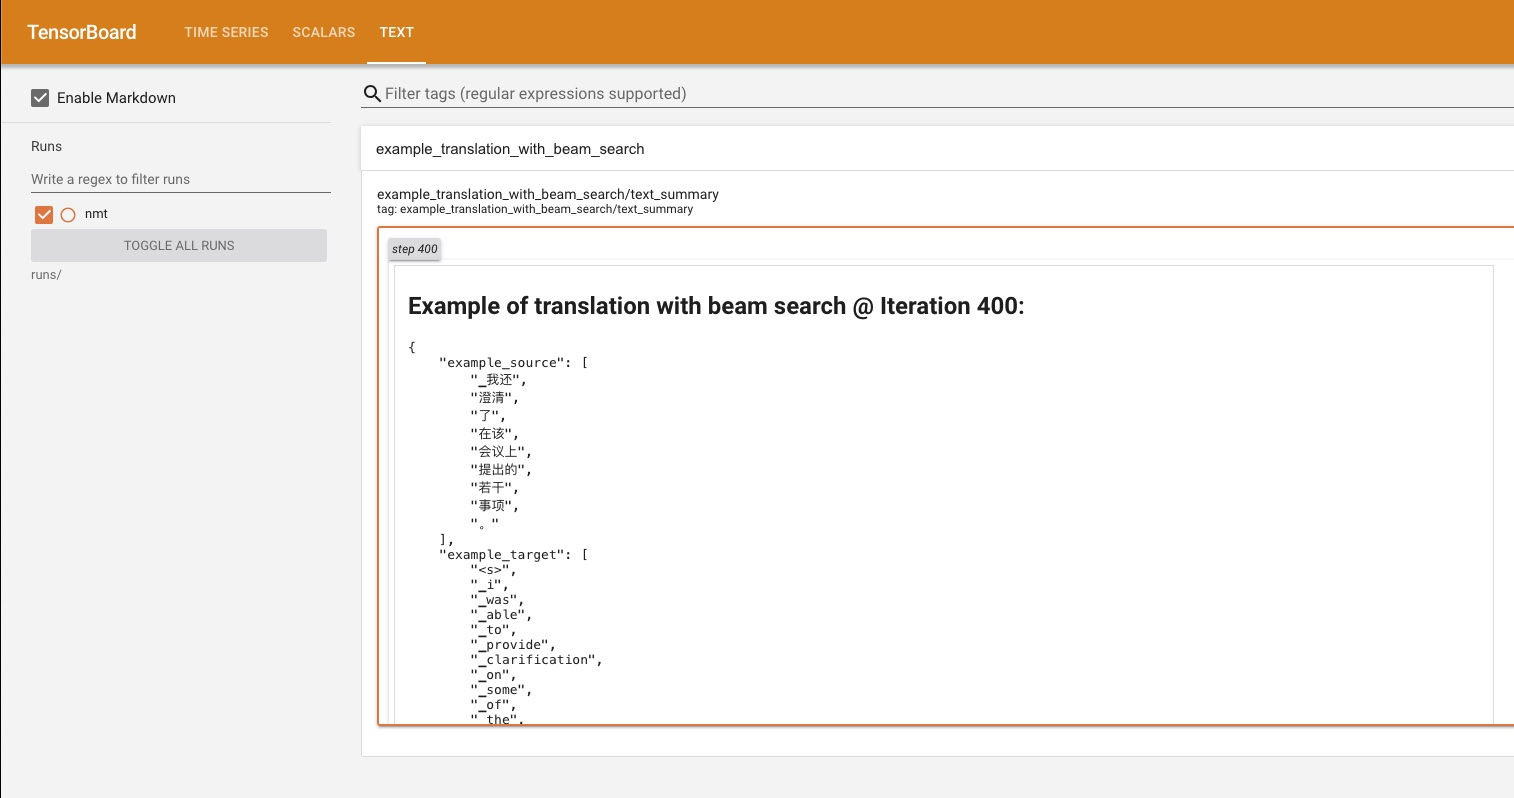
\includegraphics[width=0.7\textwidth]{images/example_translation_beam.jpg}
        \caption{Translation with beam search results for an example sentence are recorded in tensorboard for various iterations. The same data is available in the \texttt{outputs/beam\_search\_diagnostics/} folder in your working directory.}
        \label{fig:beam-search-diagnostics-tensorboard}
    \end{figure}
    

\end{parts}
